\baitap
\begin{smallfont}
%-----Bài 1-----%
    \bt[CTST Tr.88]{
    $AB$ là tiếp tuyến của $(O)$ tại $B$ 
	\begin{enumerate}[label=\alph*)]
		\item 
		Tính bán kính $r$ của $(O)$.
		\item 
		Tính chiều dài cạnh $OA$ của tam giác $ABO$.
	\end{enumerate}
    \textbf{\textit{Gợi ý:}}
    \begin{enumerate}[label=\alph*)]
		\item 
		Có tiếp tuyến nên sẽ có vuông góc, mà đề lại yêu cầu tính cạnh, vậy ta sẽ dùng định lý Pythagoras.
		\item 
		Khi tìm được đáp án của câu a ta sử dụng cộng cạnh với cạnh để tìm $OA$.
	\end{enumerate}
    }
%-----Hình bài 1-----%
\begin{marginfigure}|-4.5cm|
		\centering
		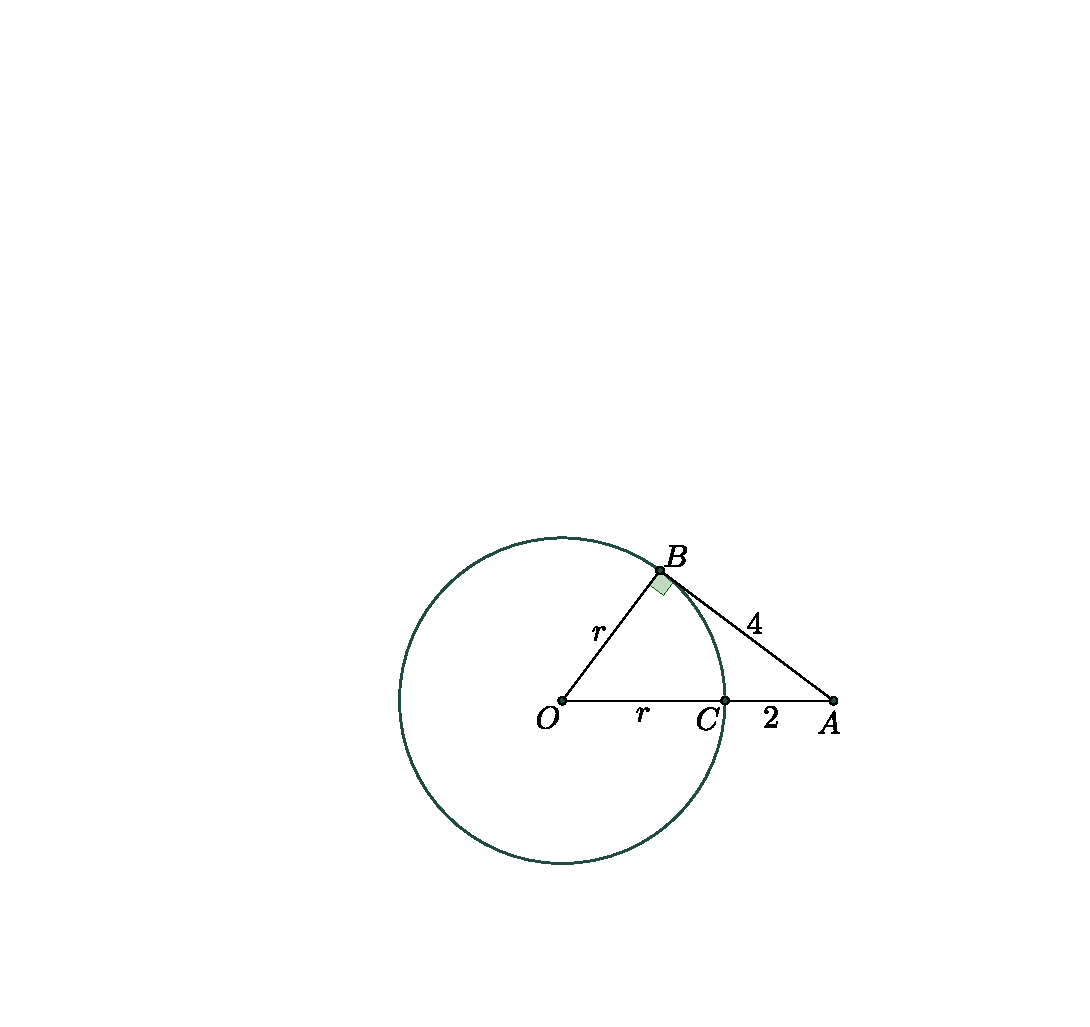
\includegraphics[width=0.7\marginparwidth]{imgc2/Bai1.pdf}
		\vspace{0.2cm}
		\margincaption{Bài 1}
		\label{hinh2.7}
\end{marginfigure}
\xdd

%-----Bài 2-----%
\bt[CTST Tr.88]{
    $MB$, $MC$ lần lượt là tiếp tuyến của đường tròn $(O)$ tại $B, C$; $\goc{COB} = 130^\circ $. Tính số đo $\goc{CMB}$. \xd
    \textbf{\textit{Gợi ý:}} \xd
    Có tiếp tuyến nên có vuông góc từ đó biết được số đo của 2 góc $B, C$ là $90^\circ$. Mà $\goc{CMB}$ nằm trong tứ giác $OBMC$. Vậy ta sẽ sử dụng tổng 4 góc trong tứ giác.
}
%-----Hình bài 2-----%
\begin{marginfigure}|-3.5cm|
		\centering
		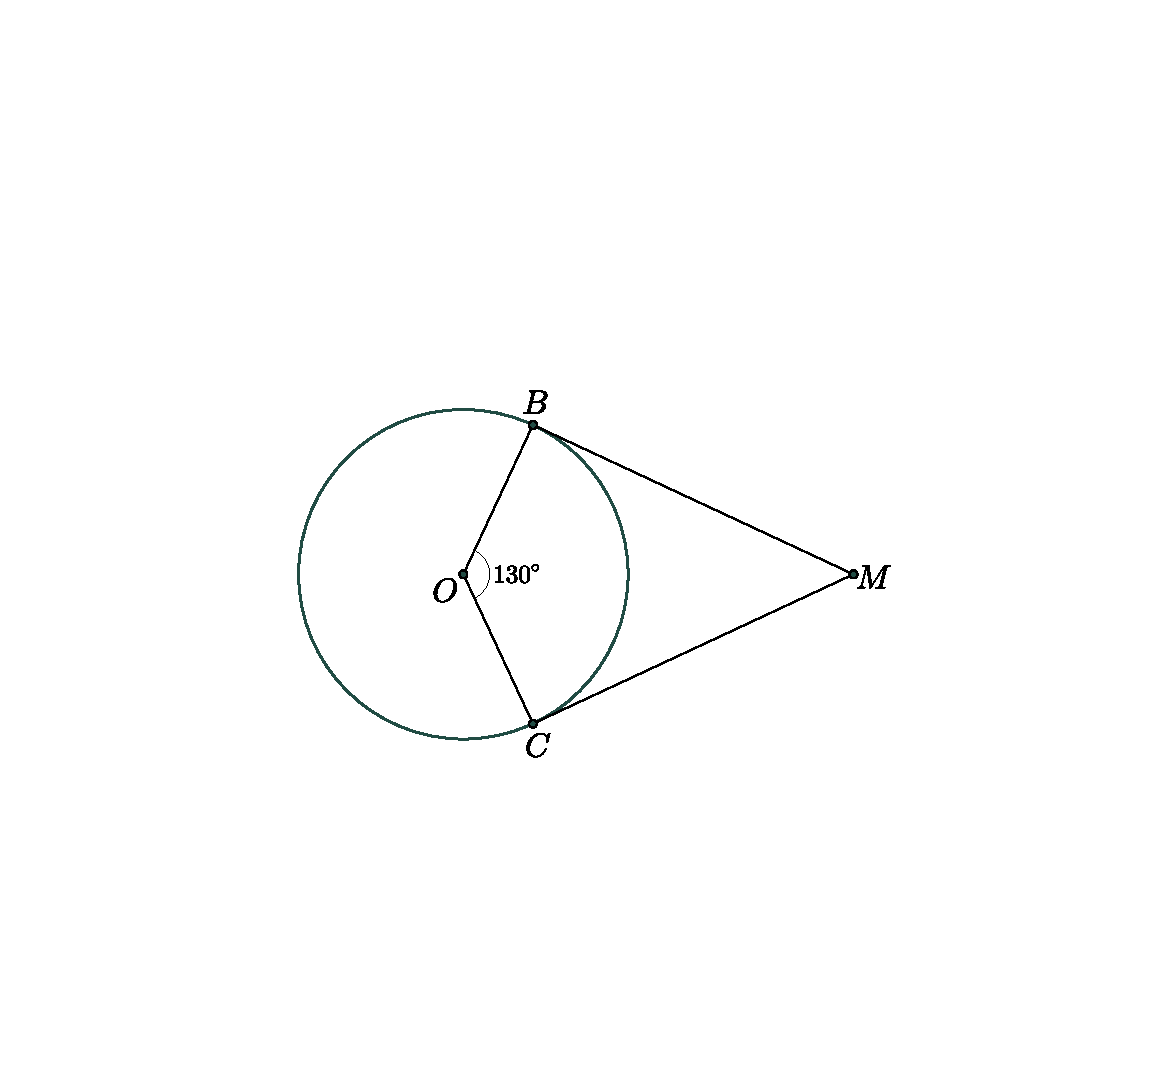
\includegraphics[width=0.8\marginparwidth]{imgc2/Bai2.pdf}
		\vspace{0.2cm}
		\margincaption{Bài 2}
		\label{hinh2.8}
\end{marginfigure}
\xdd
%-----Bài 3-----%
\bt[CTST Tr.88]{
    Biết $AB$, $AC$ lần lượt là tiếp tuyến của đường tròn $(O)$ tại $B, C$. Tính giá trị của $x$. \xd
    \textbf{\textit{Gợi ý:}} \xd
    Nhận thấy 2 tiếp tuyến $AB, AC$ cắt nhau tại $A$ nên ta sử dụng tính chất 2 tiếp tuyến cắt nhau.
    }
%-----Hình Bài 3-----%
\begin{marginfigure}|-3cm|
		\centering
		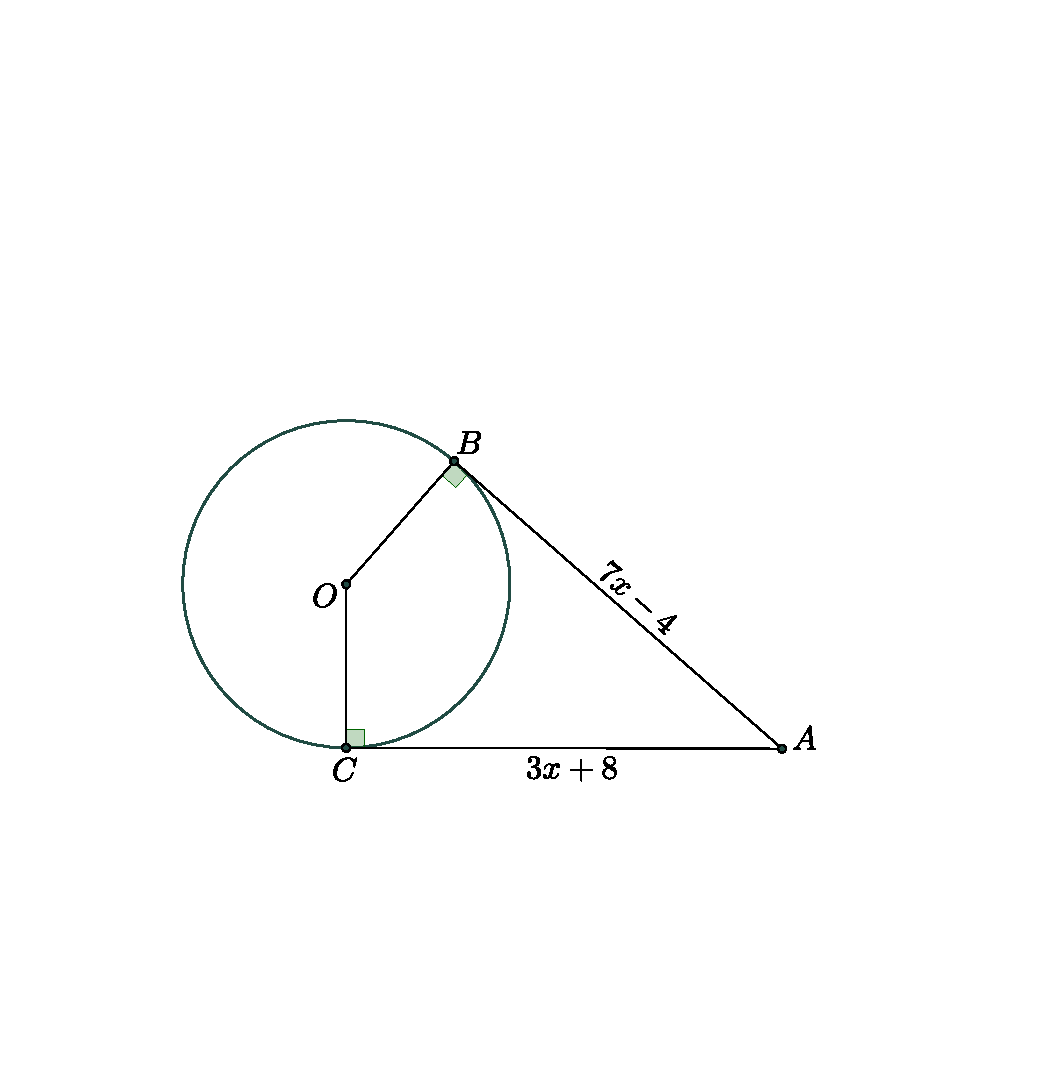
\includegraphics[width=0.8\marginparwidth]{imgc2/Bai3.pdf}
		\vspace{0.2cm}
		\margincaption{Bài 3}
		\label{hinh2.9}
\end{marginfigure}
\xdd

%-----Bài 4-----%
\bt[CTST Tr.89]{
    $AB = 9, BC = 12, AC = 15$ và $BC$ là đường kính của đường tròn $(O)$. Chứng minh $AB$ là tiếp tuyến của đường tròn $(O)$. \xd
	\textbf{\textit{Gợi ý:}} \xd
    \textbullet Khi đề bài cho 3 cạnh của một tam giác thì đó không phải sự ngẫu nhiên mà đề bài muốn ta sử dụng định lí Pythagoras đảo nhằm kiểm tra đó có phải tam giác vuông hay không. \xd
	\textbullet Để chứng minh tiếp tuyến ta chỉ có một hướng đi là chứng minh đường thẳng đó vuông góc với bán kính tại một điểm thuộc đường tròn.
	}
%-----Hình Bài 4-----%
\begin{marginfigure}|-4cm|
		\centering
		\includegraphics[width=0.7\marginparwidth]{imgc2/Bai4.pdf}
		\vspace{0.2cm}
		\margincaption{Bài 4}
		\label{hinh2.10}
\end{marginfigure}	
\xdd

\bt[CTST Tr.89]{
    Cho tam giác $ABC$ có đường tròn $(O)$ nằm trong và tiếp xúc với ba cạnh của tam giác. Biết $AM = 6~cm, BP = 3~cm, CE = 8~cm$. Tính chu vi tam giác $ABC$. \xd
    \textbf{\textit{Gợi ý:}} \xd
	\textbullet Để tính chu vi ta cần nhớ rằng "Chu vi bằng tất cả các cạnh cộng lại". Vậy để tính được chu vi $\tamgiac ABC$ ta cần tính được 3 cạnh là $AB, AC, BC$. \xd
	\textbullet Nhận thấy rằng ta có 3 tiếp tuyến với các tiếp điểm là $M, E, P$. Sử dụng tính chất 2 tiếp tuyến cắt nhau cho các cặp tiếp tuyến $(AM, AE); (BM, BP); (CE; CP)$. \xd
	\textbullet Dùng cộng cạnh hoặc trừ cạnh để tìm 3 cạnh $AB, AC, BC$.
	}
%-----Hình Bài 5-----%
\begin{marginfigure}|-4cm|
		\centering
		\includegraphics[width=0.8\marginparwidth]{imgc2/Bai5.pdf}
		\vspace{0.2cm}
		\margincaption{Bài 5}
		\label{hinh2.11}
\end{marginfigure}	
\xdd

\bt[CTST Tr.89]{
    Cho đường tròn $(O; R)$ có đường kính $AB$. Vẽ dây $AC$ sao cho $AC = R$. Gọi $I$ là trung điểm của dây $AC$. Đường thẳng $OI$ cắt tiếp tuyến $Ax$ tại $M$. Chứng minh rằng:
	\begin{enumerate}[label=\alph*)]
		\item  
		$\goc{ACB}$ có số đo bằng $90^\circ$, từ đó suy ra độ dài của $BC$ theo $R$;
		    
		\item
		$OM$ là tia phân giác của $\goc{COA}$;
		
		\item
		$MC$ là tiếp tuyến của đường tròn $(O; R)$.
	\end{enumerate}
}
\xdd

\bt[CTST Tr.89]{
    Cho đường tròn $(O; 5~cm)$, điểm $M$ nằm ngoài $(O)$ sao cho hai tiếp tuyến $MA$ và $MB$ ($A, B$ là hai tiếp điểm) vuông góc với nhau tại M
	\begin{enumerate}[label=\alph*)]
		\item  
		Tính độ dài của $MA$ và $MB$.
		
		\item
		Qua giao điểm $I$ của đoạn thẳng $MO$ và đường tròn $(O)$, vẽ một tiếp tuyến cắt $OA, OB$ lần lượt tại $C, D$. Tính độ dài của $CD$.
	\end{enumerate}
}
\xdd

\bt[CTST Tr.89]{
    Cho đường tròn $(O)$, điểm $M$ nằm ngoài $(O)$ sao cho $MA$ và $MB$ là hai tiếp tuyến ($A, B$ là hai tiếp điểm) thoả mãn $\goc{AMB} = 60^\circ$. Biết chu vi tam giác $MAB$ là $18~cm$, tính độ dài dây $AB$.
}
\end{smallfont}

\subsection{Dạng 1: Chứng minh một đường thẳng là tiếp tuyến}
\begin{smallfont}
	\bt[TOANMATH]{Cho tam giác $ABC$ có $AB = 6cm, AC = 8cm, BC = 10cm$. Vẽ đường tròn $(B; BA)$. Chứng minh $AC$ là tiếp tuyến của đường tròn $(B)$.}
	\xdd
	
	\bt[Tiến Sĩ Trần Hoan]{Cho $\tamgiac$ $ABC$ có $AB= 3cm; AC = 4cm; BC = 5cm$. Chứng minh rằng $AC$ là tiếp tuyến của đường tròn $(O)$.}
	\xdd
	
	\bt[Tiến Sĩ Trần Hoan]{Từ điểm $A$ nằm ngoài $(O;R)$ vẽ tiếp tuyến $AB$ ($B$ là tiếp điểm); lấy $C$ trên đường tròn sao cho $AB = AC$. Chứng minh rằng $AC$ là tiếp tuyến của đường tròn.
	}
	\xdd
	
	\bt[Tiến Sĩ Trần Hoan]{Cho (O); vẽ dây $BC$ khác đường kính; qua $O$; kẻ đường thẳng vuông góc với $BC$ cắt tiếp tuyến tại $B$ của đường tròn ở $A$. Chứng minh rằng $AC$ là tiếp tuyến của $(O)$.}
	\xdd 

	\bt[Tiến Sĩ Trần Hoan]{Cho $(O)$; đường kính $AB$. Kẻ tiếp tuyến tại $B$ với $(O)$; trên tiếp tuyến lấy $P$. Qua $A$ kẻ đường thẳng song song với $OP$; cắt $(O)$ tại $Q$. Chứng minh $PQ$ là tiếp tuyến $(O)$.}
	\xdd 

	\bt[Thạc Sĩ Nguyễn Văn Hòa]{Từ một điểm $A$ nằm ngoài đường tròn $(O; R)$; vẽ tiếp tuyến $AB$($B$ là tiếp điểm). Kẻ dây $BC$ vuông góc với $OA$. Chứng minh $AC$ là tiếp tuyến của đường tròn.}
	\xdd
	
	\bt[Thạc Sĩ Nguyễn Văn Hòa]{Cho đường tròn tâm $O$ và đường kính $AB$. Một điểm $M$ nằm trên đường thẳng $AB$ ($A$ nằm giữa $M$ và $B$), qua điểm $M$ kẻ đường thẳng $MC$ tiếp xúc với đường tròn $(O)$ tại $C$. Từ $O$ dựng đường vuông góc với $BC$ cắt $MC$ tại $N$. Chứng minh đường thẳng $NB$ là tiếp tuyến của $(O)$.}
	\xdd 

	\bt[Thạc Sĩ Nguyễn Văn Hòa]{Cho 3 điểm $A; B; C$ cùng thuộc (O) sao cho $\tamgiac ABC$ cân tại $A$. Vẽ hình bình hành $ABCD$. Chứng minh $AD$ là tiếp tuyến của $(O)$.}
	\xdd 

	\bt[Internet]{Cho tam giác $ABC$ cân tại $A$ đường cao $BH$. Trên mặt phẳng chứa $C$ bờ $AB$ vẽ $Bx \vuong BA$ cắt đường tròn tâm $B$ bán kính $BH$ tại $D$. Chứng minh $CD$ là tiếp tuyến của $(B)$.}
	\xdd

	\bt[Internet]{Cho hình thang vuông $ABCD; (\goc{A}=\goc{B}=90^\circ)$ có $O$ là trung điểm của $AB$ và góc $\goc{COD} = 90^\circ$. Chứng minh $CD$ là tiếp tuyến của đường tròn đường kính $AB$.}
\end{smallfont}
